% !TEX encoding = UTF-8 Unicode
\documentclass[
11pt,
master, % тип документа
subf, % подключить и настроить пакет subfig для вложенной нумерации рисунков
href, % подключить и настроить пакет hyperref
colorlinks=true, % цветные гиперссылки
%fixint=false % отключить прямые знаки интегралов
]{disser}
\usepackage[
  a4paper, mag=1000,
  left=2.5cm, right=1cm, top=2cm, bottom=2cm, headsep=0.7cm, footskip=1cm
]{geometry}
\usepackage[T2A]{fontenc}
\usepackage[utf8]{inputenc}
\usepackage[english,russian]{babel}
\usepackage{pdfpages}
\ifpdf\usepackage{epstopdf}\fi
\usepackage{hyperref}
\usepackage{epstopdf}
\usepackage{amsmath}
\usepackage{amssymb}
\usepackage{lastpage} % счётчик страниц
\usepackage{setspace}

% Полуторный интервал
%\usepackage[nodisplayskipstretch]{setspace}
%\onehalfspacing

\graphicspath{{Img/}}
\DeclareGraphicsExtensions{.pdf,.png,.jpg}


% Номера страниц снизу и по центру
\pagestyle{footcenter}
\chapterpagestyle{footcenter}

% Включать подсекции в оглавление
\setcounter{tocdepth}{2}

\newcommand*{\PartDif}[2]{\frac{\partial #1}{\partial #2}}
\newcommand*{\PartDiff}[2]{\frac{\partial^2 #1}{\partial #2^2}}
\newcommand*{\PartD}[1]{\frac{\partial}{\partial #1}}
\newcommand*{\SR}[1]{\left( #1 \right)}
\newcommand*{\Ap}[2]{\hat{#1}_{#2}}
\newcommand*{\Apr}[2]{#1_{#2}}

\newenvironment{itemize*}
  {\begin{itemize}%
    \setlength{\itemsep}{1pt}
    \setlength{\parskip}{1pt}}
  {\end{itemize}}

\newenvironment{enumerate*}
  {\begin{enumerate}%
    \setlength{\itemsep}{1pt}
    \setlength{\parskip}{1pt}}
  {\end{enumerate}}

\begin{document}

\begin{titlepage}
\begin{center}
{
\footnotesize\setstretch{1.0}
Федеральное государственное бюджетное образовательное учреждение высшего образования\\
<<Московский государственный технический университет имени Н.Э. Баумана\\ (национальный исследовательский университет)>>\\(МГТУ им. Н.Э. Баумана)\\
}
\end{center}
\begin{figure}[h!]
    \begin{minipage}[b]{0.9\textwidth}\setstretch{1.5}
        \centering
        Факультет <<Фундаментальные науки>>\\
        Кафедра <<Физика>> ФН4\\\vspace{1.7cm}
    \end{minipage}
\end{figure}

\begin{flushright}
    На правах рукописи\\
    УДК 53.043; 538.931
\end{flushright}

\vspace{10mm}

\begin{center}
    \textbf{КУРСОВАЯ РАБОТА}\\
    \vspace{5mm}
    \textbf{<<Моделирование загрязнения чувствительной поверхности оптической системы продуктами газовыделения материала покрытия бленды>>}
    
\end{center}

\vspace{40mm}

\begin{table}[h]
    \begin{tabular}{lll}
    Студент\hspace{4cm} & \underline{\hspace{4cm}}  &  \hspace{2cm}Хижик А.И.\\ \\
    Научный руководитель \\доцент, к.ф.-м.н. & \underline{\hspace{4cm}} & \hspace{2cm}Хасаншин Р.Х.
    \end{tabular}
\end{table}

\vspace{50mm}

\begin{center}
    Москва -- 2020
\end{center}
\end{titlepage}

\setcounter{page}{2}
\addtocontents{toc}{~\hfill\textbf{Стр.}\par}
\setcounter{chapter}{0}
\setcounter{section}{1}

\tableofcontents

\newpage
\begin{center}
	\textbf{\Large Постановка задачи}
\end{center}

\addcontentsline{toc}{chapter}{Постановка задачи}

~

Рассчитать распределение продуктов газовыделения по диаметру оптической поверхности. Угловое распределение молекул покидающих поверхность материала покрытия считать изотропным.

\begin{figure}[h]
	\centering
	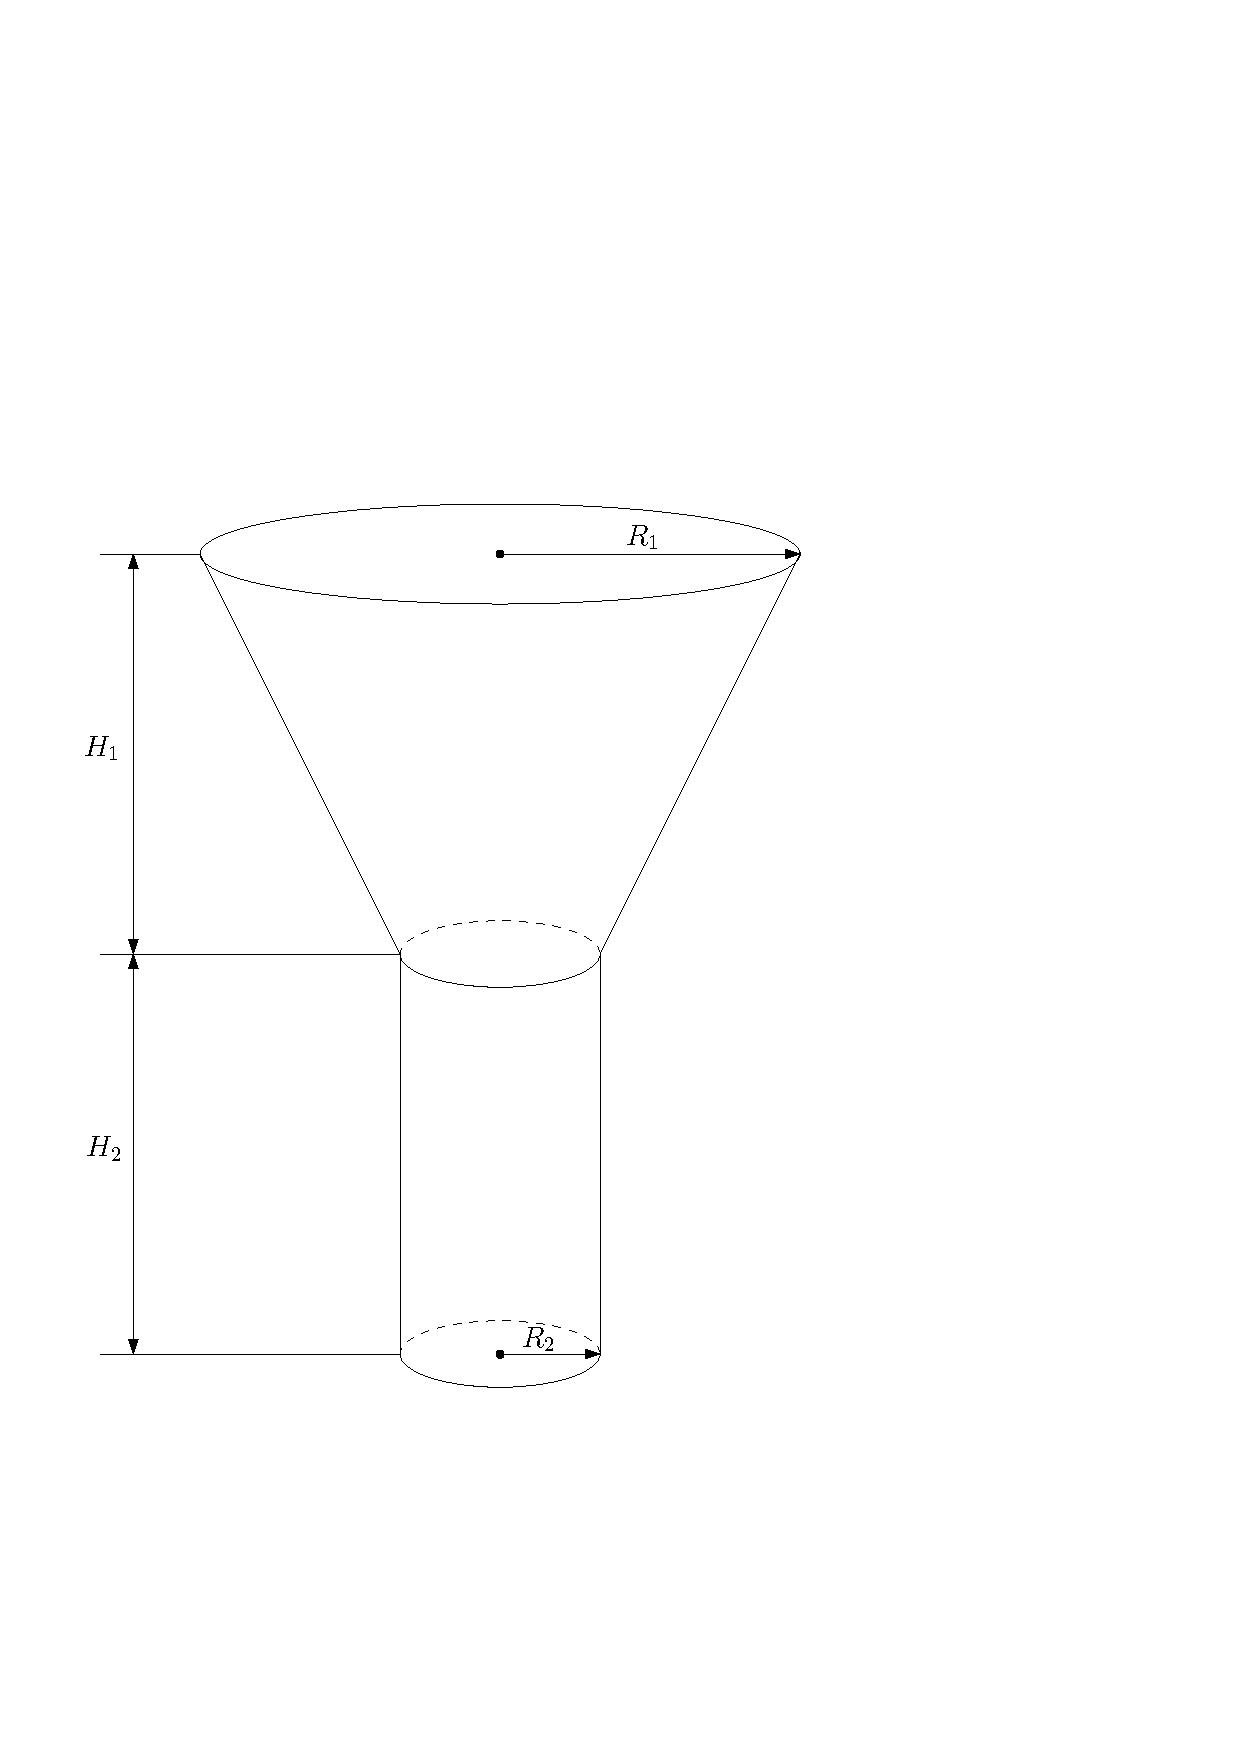
\includegraphics[width=0.3\linewidth]{pic}
	\caption{}
\end{figure}
\begin{align}
	&\PartDif{C(x,t)}{t} = \PartD{x}\SR{D(x,t)\PartDif{C(x,t)}{x}} - \beta C(x,t), \;\; 0 < x < h, \;\; 0 < t < 1000, \label{eq:1}\\
	&C(x,t)\bigg|_{t = 0} = C_0, \label{eq:2}\\
	&\SR{\PartDif{C(x,t)}{x}}\bigg|_{x = 0} = 0, \label{eq:3}\\
	&\SR{D(x,t)\PartDif{C(x,t)}{x} + k(t)C(x,t)}\bigg|_{x = h} = 0, \label{eq:4}
\end{align}
где $D(x) = D_0\SR{1 + \frac{x}{h}}$, $D_0 = 0.002$ мкм$^2\cdot$с$^{-1}$, $k = 0.01$ мкм$\cdot$с$^{-1}$, $C_0 = 1$ моль$\cdot$мкм$^{-3}$, $R_1 = 5.0 \cdot 10^{5}$ мкм, $R_2 = 2.0 \cdot 10^5$ мкм, $\beta = 10^{-6}$ с$^{-1}$, $h = 100$ мкм, $H_1 = 10^6$ мкм, $H_2 = 5 \cdot 10^5$ мкм.\\
$C(x,t)$ -- пространственно-временное распределение концентрации потенциальных продуктов газовыделения (ППГ) в материале;\\
$C_0$ -- начальная концентрация ППГ в материале;\\
$h$ -- толщина внутреннего покрытия из полимерного материала;\\
$D_0$ -- эффективный коэффициент диффузии ППГ в материале;\\
$k$ -- эффективный коэффициент десорбции ППГ с поверхности материала;\\
$\beta$ -- эффективная скорость химической реакции с участием ППГ;\\
$R_1,$ $R_2$, $H_1$, $H_2$ -- размеры бленды.


\newpage
\begin{center}
	\textbf{\Large Моделирование потери массы ПКМ}
\end{center}

\addcontentsline{toc}{chapter}{Моделирование потери массы ПКМ}

~

\subsection{Физико-математическая модель}
Для изучения потери массы полимерного композита при вакуумно-тепловом воздействии в качестве модельных материалов возьмём терморегулирующие покрытия, занимающие большую площадь поверхности КА и являющиеся одними из основных источников продуктов СВА. В модели, описывающей потерю массы образца такого материала, нанесённого на металлическую подложку, постулируется, что изменение концентрации $C_m(x,t)$ $m$-го компонента газовыделения (молекулы или атома) в материале при вакуумно-тепловом воздействии обусловлено следующими процессами \cite{Khas06, Khas06i}:
\begin{enumerate}
	\item Десорбцией адсорбированных летучих веществ $m$-го вида с поверхности материал-вакуум;
	\item Химическими реакциями с участием $m$-ой компоненты;
	\item Сублимацией материала с поверхности материал-вакуум;
	\item Диффузией и десорбцией летучих веществ $m$-го вида, абсорбированных или образованных в нём в результате термической деструкции.
\end{enumerate}
Также постулируется, что скорость потери массы $\dot{M}_m(t)$ соответствующая ЛВ $m$-го типа пропорциональна его концентрации в приповерхностном слое ПМ $C_m(h-vt, t)$:
$$\dot{M}_m(t) = m_m \SR{k_m(t) + v(t)} C_m(l-v(t) t,t),$$
где $m_m$ -- масса молекул ЛВ $m$-го типа, $v(t)$ -- скорость сублимации, $h$ -- толщина материала,\\
 $k_m(t)$ -- эффективный коэффициент десорбции ЛВ $m$-го типа.

Тогда суммарная потеря массы с единицы поверхности материала $M_{total}(t)$ за время $t$ вычисляется по следующей формуле:
$$M_{total} = \sum_{m=1}^{M} M_m(t) = \sum_{m=1}^{M}m_m \int_{0}^{t} \SR{k_m(\tau) + v(\tau)} C_m(l-v(\tau) \tau,\tau) d\tau,$$
где $M$ -- число типов ЛВ в облучённом материале.

При рассмотрении перечисленных процессов в объёме и на их поверхности композиционного материала со сложной энергетической структурой возможен только макроскопический подход. Поэтому далее используются эффективные коэффициенты диффузии, десорбции, термической деструкции и скорости химических реакций -- параметры, с помощью которых описываются процессы, наблюдаемые при лабораторных и натурных экспериментах.

Концентрации $C_m(x,t)$, $m = \overline{1,M}$ компонентов газовыделения в ПКМ в рамках выше сформулированных предположений, описываются системой нелинейных дифференциальных уравнений в частных производных:
\begin{align}
	&\PartDif{C_m(x,t)}{t} = \PartD{x}\SR{D_m(x,t) \PartDif{C_m(x,t)}{x}} - \beta_m(x,t) C_m(x,t) + S_m(x,t), \label{eq:moe1}\\
	&x \in (0, h-v t), \;\; t>0, \;\; v(t) t < h, \nonumber \\
	&C_m(x,t)\bigg{|}_{t = 0} = R_m(x),\;\; x \in [0,h], \label{eq:moe2}\\
	&\SR{D_m(x,t)\PartDif{C_m(x,t)}{x} + \left(k_m(t) + v(t)\right) C_m(x,t)}\bigg{|}_{x = h - v t} = \frac{\partial C_m(x,t)}{\partial x}\bigg{|}_{x = 0} = 0, \label{eq:moe3}
\end{align}
где $\beta_m(x,t)$ -- обобщённая скорость реакций первого порядка с участием $m$-й компоненты;\\
$R_m(x)$ -- концентрация ЛВ $m$-го вида в материале в начальный момент времени;\\
$D_m(x,t)$ -- эффективный коэффициент диффузии ЛВ $m$-го вида;\\
$S_m(x,t)$ -- функция источника $m$-й компоненты.\\

\subsection{Моделирование осаждения ЛВ на оптические поверхности}
Элементарное решение задачи \eqref{eq:moe1}-\eqref{eq:moe3} при следующих параметрах модели: температура материала постоянна и все коэффициенты уравнений являются константами $R_m(x) = R_m$, $D_m(x,t) = D_m$, $k_m(t) = k_m$, $\beta_m(x) = \beta_m$, $v(t) = 0$, будет иметь следующий вид
\begin{align}\label{eq:moesol}
	&C_m(x,t) = 2\sum_{n=1}^{\infty}\frac{\left(\lambda_{mn} D^2_m + k^2_m\right) \cos\left(\sqrt{\lambda_{mn}} x\right)}{k_m D_m + h\left(\lambda_{mn} D^2_m + k^2_m\right)} \exp\SR{-\left(\beta_m + D_m \lambda_{mn}\right) t} \cdot \\
	&\cdot \SR{\frac{R_m \sin\left(\sqrt{\lambda_{mn}} h\right)}{\sqrt{\lambda_{mn}}} + \int_{0}^{t}\int_{0}^{h} S_m(x,\xi) \cos\left(\sqrt{\lambda_{mn}} x\right) \exp\SR{\xi \left(\beta_m + D_m \lambda_{mn}\right)} dx d\xi}, \nonumber
\end{align}
где $\lambda_{mn} > 0$ -- решение трансцендентного уравнения
$$\sqrt{\lambda_{mn}} \mathrm{tg}\left(\sqrt{\lambda_{mn}} h\right) = \frac{k_m}{D_m}.$$




Рассмотрим процесс осаждения потенциальных продуктов газовыделения (ППГ) на оптическую поверхность. На рис. \ref{plm1} представлена металлическая бленда, в основании которой находится оптика. В силу того, что металлический корпус защищает её внутреннюю поверхность от излучения: $S(x,t) = 0$.
\begin{figure}[htbp]
	\centering{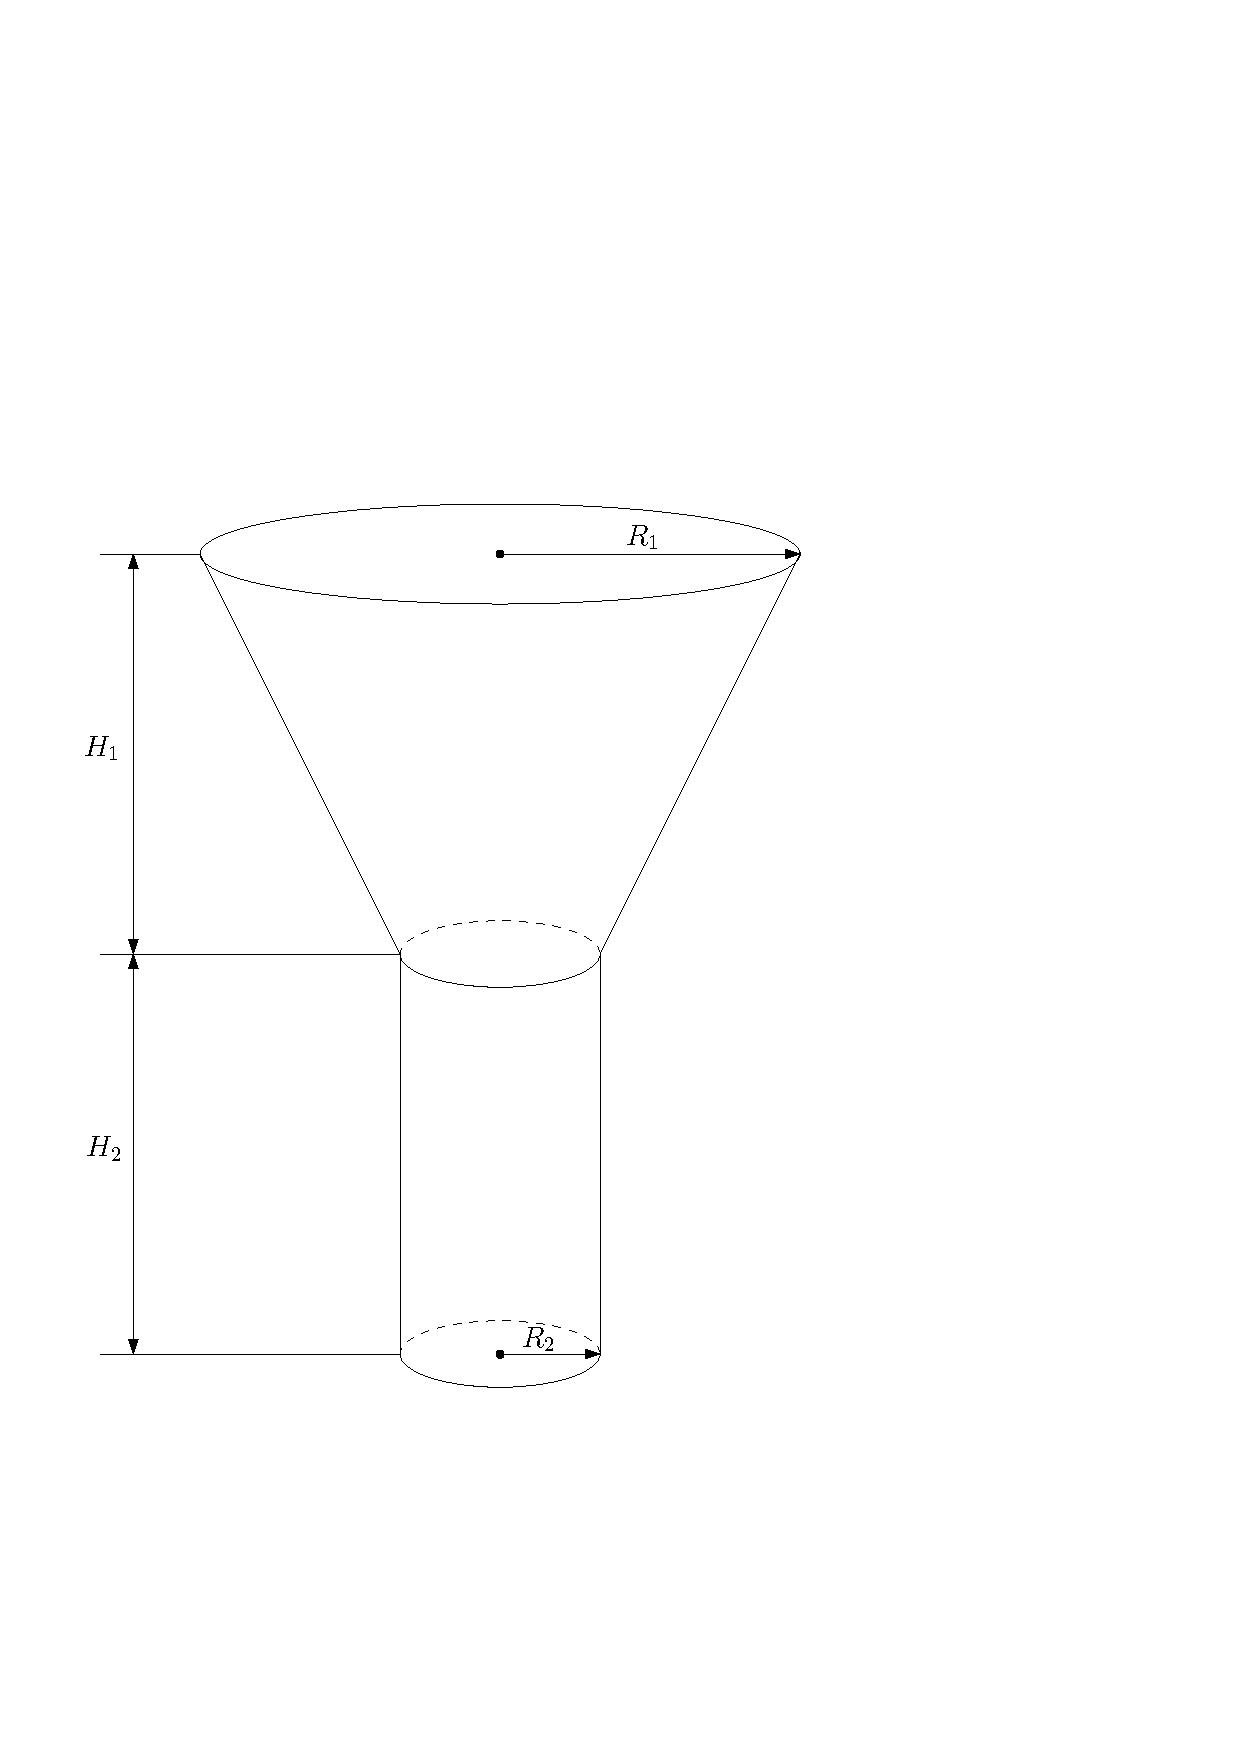
\includegraphics[width=0.3\linewidth]{pic}}
	\caption{Бленда.}\label{plm1}
\end{figure}

Для расчётов так же как в предыдущем разделе выберем следующие параметры модели: $D_0 = 0.002$  мкм$^2\cdot$с$^{-1}$ -- эффективный коэффициент диффузии ППГ в материале, $k = 0.01$ мкм$\cdot$с$^{-1}$ -- эффективный коэффициент десорбции ППГ с поверхности материала, $\beta = 10^{-6}$ с$^{-1}$ -- эффективная скорость химической реакции с участием ППГ, $R = 1$ моль$\cdot$мкм$^{-3}$ -- начальная концентрация ППГ в материале, $h = 100$ мкм -- толщина внутреннего покрытия из полимерного материала, $R_1 = 5.0 \cdot 10^{5}$ мкм, $R_2 = 2.0 \cdot 10^5$ мкм, $H_1 = 10^6$ мкм, $H_2 = 5 \cdot 10^5$ мкм -- размеры бленды. Система уравнений \eqref{eq:moe1}-\eqref{eq:moe3}, описывающая распределение ППГ в материале бленды, принимает следующий вид:
\begin{align}
	&\PartDif{C(x,t)}{t} = \PartD{x}\SR{D(x)\PartDif{C(x,t)}{x}} - \beta C(x,t), \;\; 0 < x < h, \;\; 0 < t < 1000, \label{eq:m1}\\
	&C(x,t)\bigg|_{t = 0} = R, \label{eq:m2}\\
	&\SR{D(x)\PartDif{C(x,t)}{x} + k C(x,t)}\bigg|_{x = h} = \SR{\PartDif{C(x,t)}{x}}\bigg|_{x = 0} = 0, \label{eq:m3}
\end{align}
где $D(x) = D_0\left(1 + \frac{x}{h}\right)$, $C(x,t)$ -- пространственно-временное распределение концентрации ППГ в материале.

\subsubsection{Численное решение}

\begin{figure}[h]
	\centering
	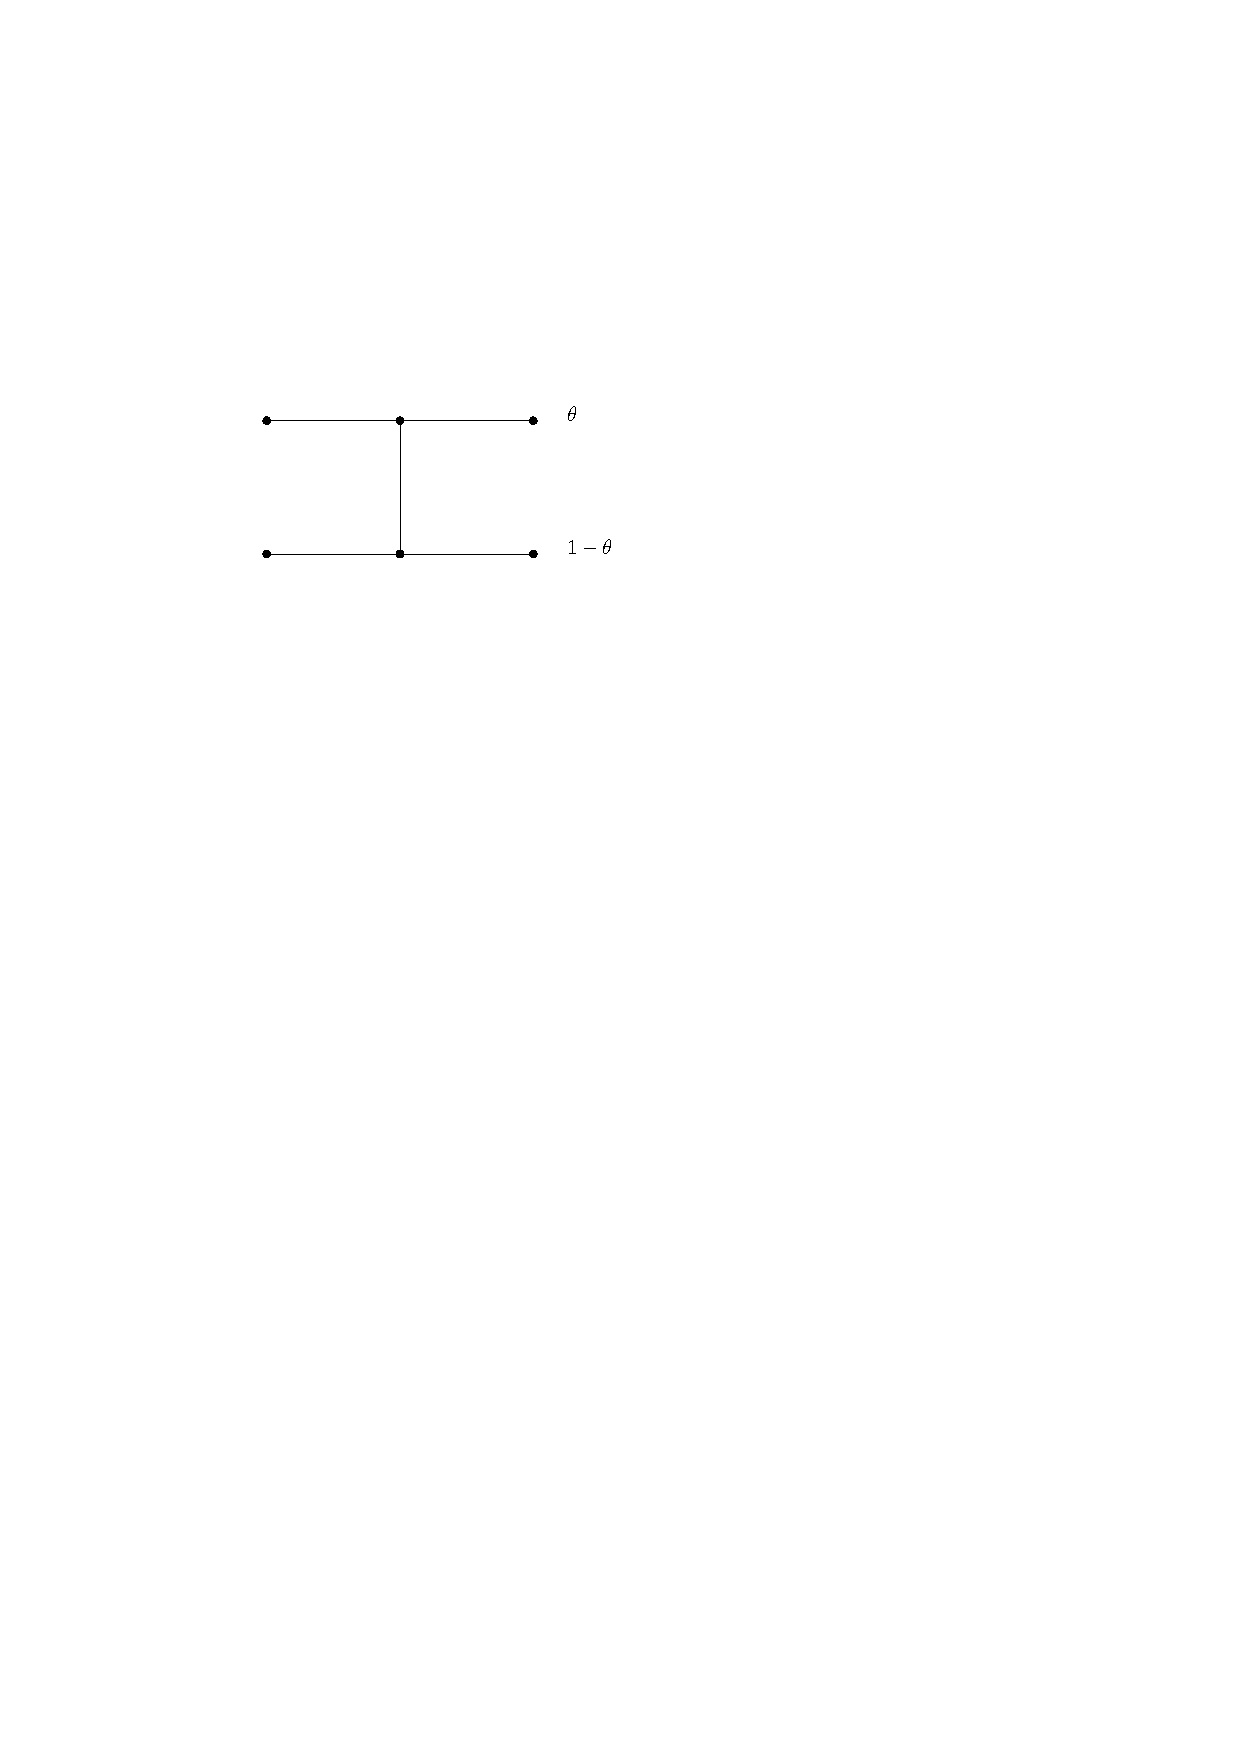
\includegraphics[width=0.45\linewidth]{pic1}
	\caption{Расположение узлов разностной схемы}\label{ris:1}
\end{figure}

Разностная схема для задачи  \eqref{eq:m1}-\eqref{eq:m3}:
\begin{align}
	&-\Ap{A}{i} \Ap{u}{i-1} + \Ap{C}{i} \Ap{u}{i} - \Ap{B}{i} \Ap{u}{i+1} = \Ap{F}{i}, \;\; i = \overline{1,N_{x}-1}, \label{eq:9.0}\\
	& u^0_i = C_0, \label{eq:9.1}\\
	& \Ap{u}{0} = \Ap{\varkappa}{1} \Ap{u}{1} + \Ap{\nu}{1},\;\; \Ap{u}{N_{x}} = \Ap{\varkappa}{2} \Ap{u}{N_{x} -1} + \Ap{\nu}{2}, \label{eq:9.2}
\end{align}
где
{\small
\begin{align}
		&\Ap{A}{i} = \theta \Ap{\alpha}{i - \frac{1}{2}}, ~~~ \Ap{C}{i} = 1 + \theta \left(\Ap{\alpha}{i + \frac{1}{2}} + \Ap{\alpha}{i - \frac{1}{2}}\right), ~~~ \Ap{B}{i} = \theta \Ap{\alpha}{i + \frac{1}{2}} , \label{eq:10.1}\\
		& \Ap{F}{i} = (1 - \theta) \Apr{\alpha}{i - \frac{1}{2}} \Apr{u}{i-1} + \SR{1 - (1 - \theta) \left(\Apr{\alpha}{i + \frac{1}{2}} + \Apr{\alpha}{i - \frac{1}{2}}\right) - \beta \tau} \Apr{u}{i} + (1 - \theta) \Apr{\alpha}{i + \frac{1}{2}} \Apr{u}{i+1}, \label{eq:10.4}\\
		&\Ap{\varkappa}{1} = 1, \;\; \Ap{\varkappa}{2} = \frac{\Ap{D}{N_x}}{\Ap{D}{N_x} + h}, \;\; \Ap{\nu}{1} = \Ap{\nu}{2} = 0, \;\;  \alpha(x) = \frac{\tau}{h^2} D(x). \label{eq:10.5}
\end{align}
}

Для решения трёхточечных разностных уравнений вида \eqref{eq:9.0} с краевыми условиями \eqref{eq:9.2} применяется метод прогонки.

Формулы прямой прогонки:
\begin{align}
	&\Ap{\xi}{i+1} = \frac{\Ap{B}{i}}{\Ap{C}{i} - \Ap{A}{i} \Ap{\xi}{i}},\;\; \Ap{\xi}{1} = \Ap{\varkappa}{1},\;\; i = \overline{1,N_{x} - 1}, \label{eq:11}\\
	&\Ap{\eta}{i+1} = \frac{\Ap{A}{i} \Ap{\eta}{i} + \Ap{F}{i}}{\Ap{C}{i} - \Ap{\xi}{i} \Ap{A}{i}}, \;\; \Ap{\eta}{1} = \Ap{\nu}{1},\;\; i = \overline{1,N_{x} - 1}. \label{eq:12}
\end{align}

Формулы обратной прогонки:
\begin{align}
	&\Ap{u}{N_x} = \frac{\Ap{\nu}{2} + \Ap{\varkappa}{2} \Ap{\eta}{N_{x}}}{1 - \Ap{\varkappa}{2} \Ap{\xi}{N_{x}}}, \label{eq:16}\\
	&\Ap{u}{i} = \Ap{\xi}{i+1} \Ap{u}{i+1} + \Ap{\eta}{i+1}, \;\; i = \overline{N_{x}-1, 0}. \label{eq:17}
\end{align}

\subsection{Результаты вычислений}

Считая поток изотропным, получаем, что плотность потока молекул с единицы поверхности материала равна $\Phi(t) = k \cdot C(h,t)$.

\begin{figure}[h!]
	\centering
	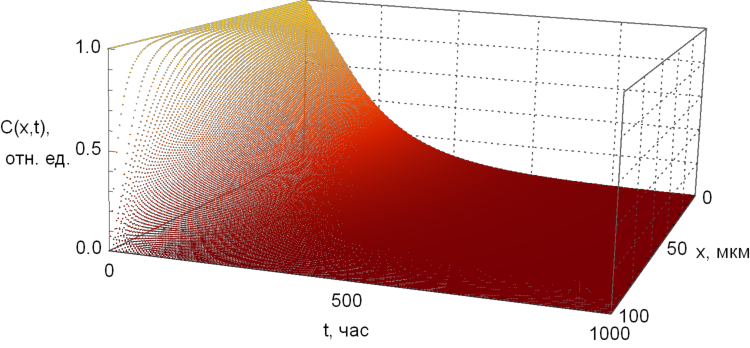
\includegraphics[width=\linewidth]{LWSrad01}
	\caption{Пространственно-временное распределение ППГ в бленде.}\label{ris:m1}
\end{figure}

В результате численного решения задачи (\ref{eq:m1}-\ref{eq:m3}), получено распределение ППГ в бленде, представленное на рис. \ref{ris:m1}.

Получим распределение частиц ППГ по поверхности оптики. Для этого решим задачу переноса частиц ППГ в бленде, используя метод Монте-Карло. На рис. \ref{ris:6} представлены распределения частиц при различных геометрических конфигурациях бленды, на рис. \ref{ris:7} -- примеры смоделированных траекторий частиц.

\begin{figure}[htbp]
	\begin{minipage}[h]{0.45\linewidth}
		\centering
		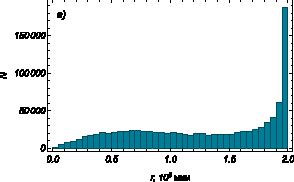
\includegraphics[width=1\linewidth]{hist_h2=0dot5}
	\end{minipage}
	\hfill
	\begin{minipage}[h]{0.45\linewidth}
		\centering
		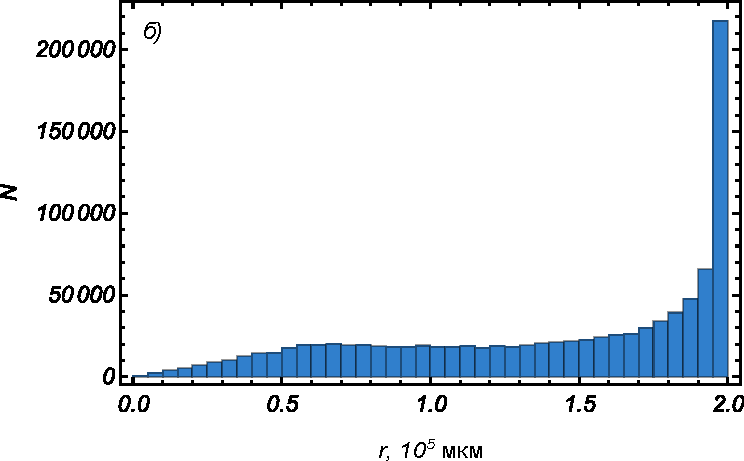
\includegraphics[width=1\linewidth]{hist_h2=1}
	\end{minipage}
	\vfill
	\begin{minipage}[h]{0.45\linewidth}
		\centering
		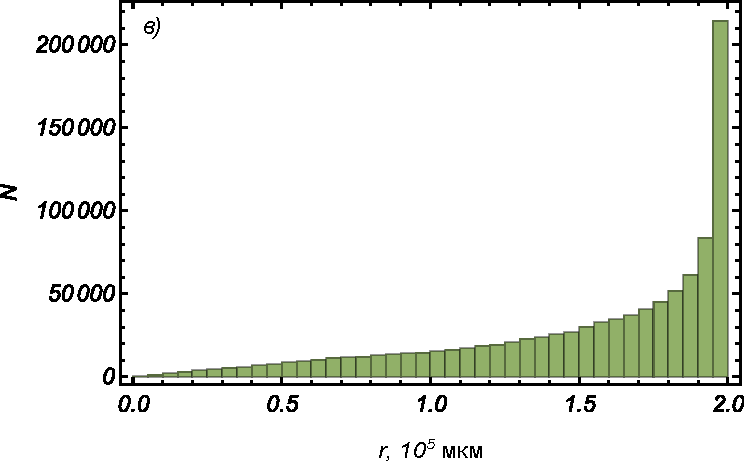
\includegraphics[width=1\linewidth]{hist_h2=2}
	\end{minipage}
	\hfill
	\begin{minipage}[h]{0.45\linewidth}
		\centering
		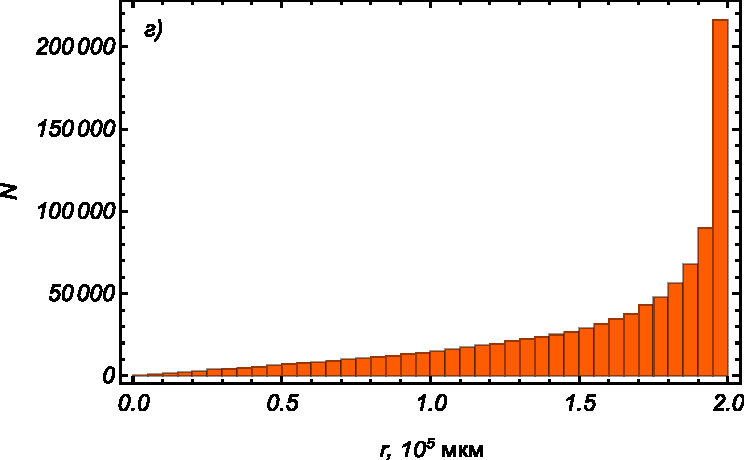
\includegraphics[width=1\linewidth]{hist_h2=5}
	\end{minipage}
	\vfill
	\begin{minipage}[h]{1\linewidth}
		\centering
		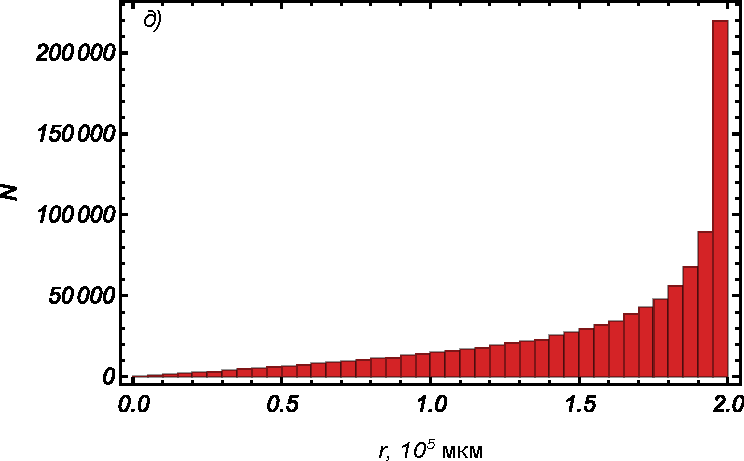
\includegraphics[width=0.45\linewidth]{hist_h2=10}
	\end{minipage}
	\vfill
	\caption{Распределения $N = 10^6$ частиц по поверхности оптики при различных значениях высоты цилиндрической части бленды \\
		а) $H_2 = 0.5 \cdot 10^5$ мкм, б) $H_2 = 1 \cdot 10^5$ мкм, в) $H_2 = 2 \cdot 10^5$ мкм, г) $H_2 = 5 \cdot 10^5$ мкм, д) $H_2 = 10 \cdot 10^5$ мкм.}
	\label{ris:6}
\end{figure}

Из рис. \ref{ris:6} видно, что с увеличением высоты цилиндрической части бленды происходит <<сглаживание>> распределения -- это результат уменьшения потока частиц, падающих на оптику напрямую с поверхности конусной части бленды.

\newpage
\begin{figure}[h!]
	\begin{minipage}[h]{0.44\linewidth}
		\centering
		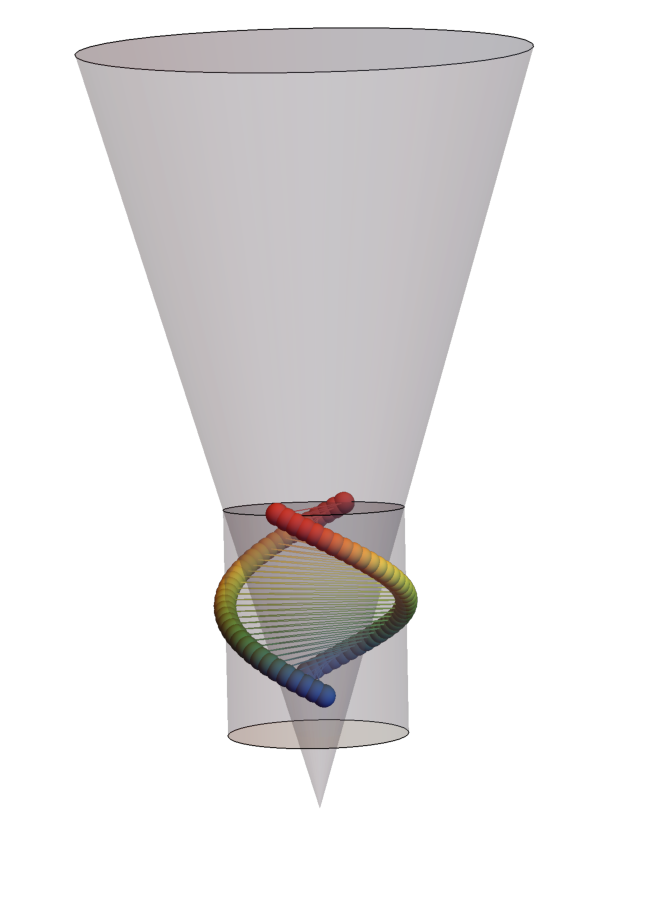
\includegraphics[width=1\linewidth]{vis1} \\ а)
	\end{minipage}
	\hfill
	\begin{minipage}[h]{0.4\linewidth}
		\centering
		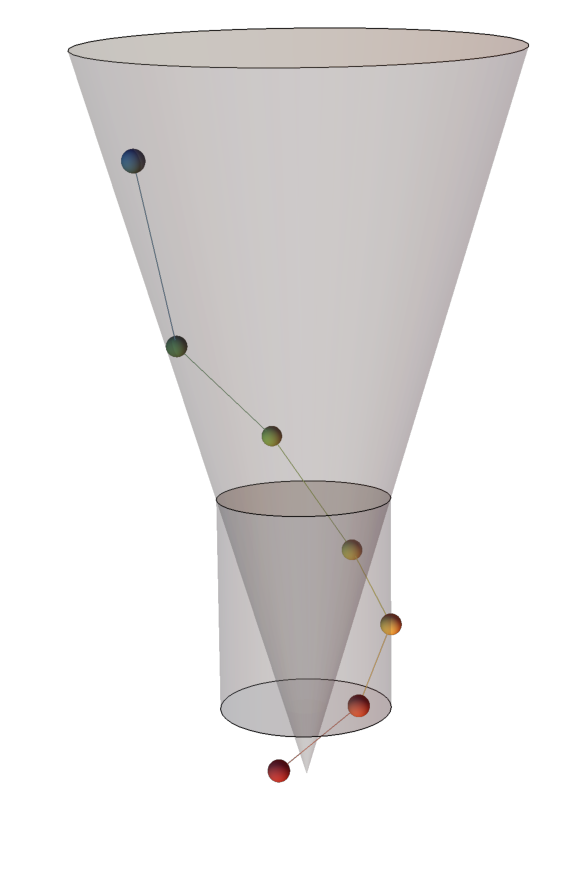
\includegraphics[width=1\linewidth]{vis2} \\ б)
	\end{minipage}
	\vfill
	\begin{minipage}[h]{0.48\linewidth}
		\centering
		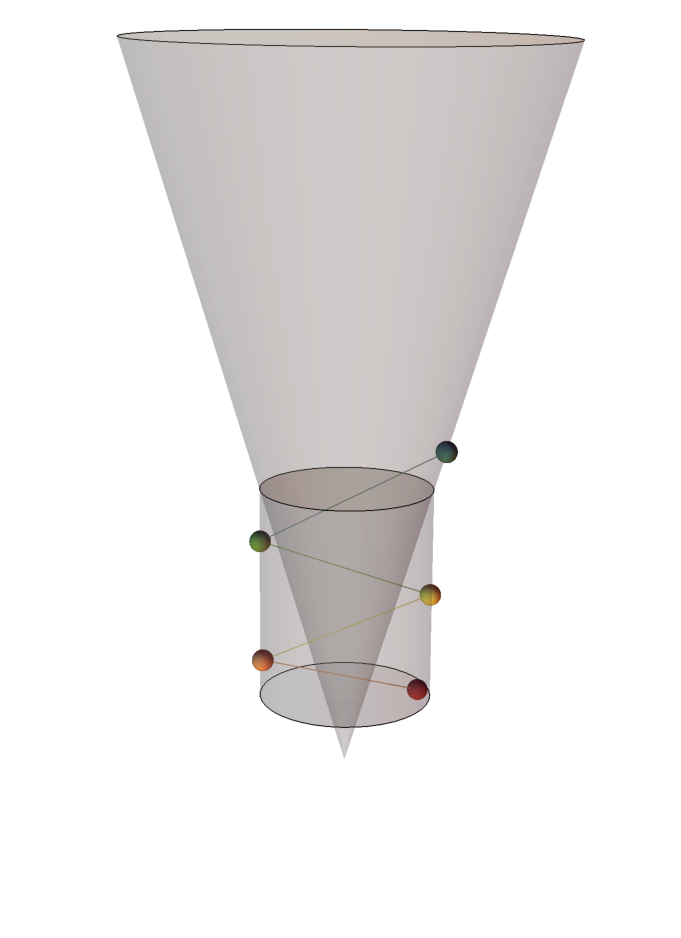
\includegraphics[width=1\linewidth]{vis3} \\ в)
	\end{minipage}
	\hfill
	\begin{minipage}[h]{0.4\linewidth}
		\centering
		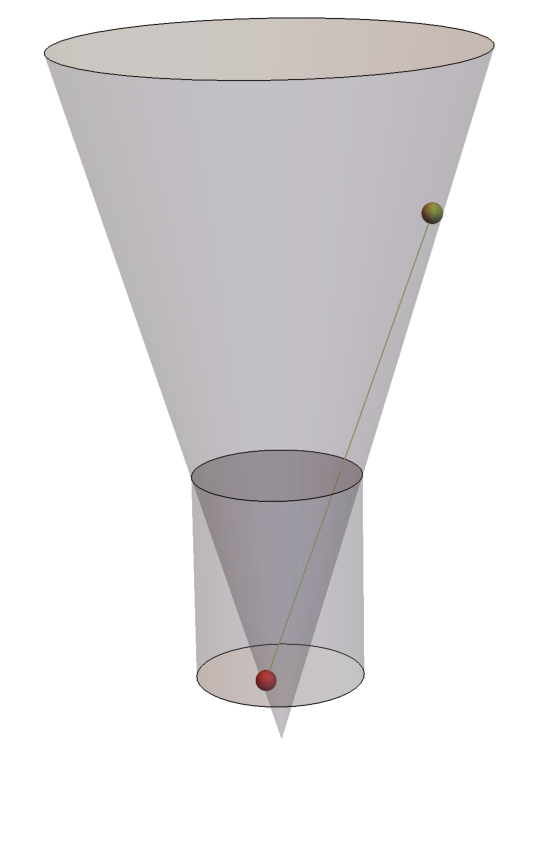
\includegraphics[width=1\linewidth]{vis4} \\ г)
	\end{minipage}
	\caption{Траекторий частиц.}
	\label{ris:7}
\end{figure}

\newpage
\textbf{Выводы}
\begin{itemize}
	\item Получено пространственно-временное распределение потенциальных продуктов газовыделения во внутреннем полимерном покрытии бленды бортового оптического прибора космического аппарата.
	\item Исследованы закономерности распределения потенциальных продуктов газовыделения по чувствительной к загрязнениям поверхности  оптического прибора для разных геометрических конфигураций бленды.
\end{itemize}

\let\BibEmph=\emph
\bibliographystyle{gost2008n}
\bibliography{Ref-Diss}
\end{document}
